\documentclass[12pt,a4paper]{article}
\usepackage[utf8]{inputenc}
\usepackage[T1]{fontenc}
\usepackage[french]{babel}
\usepackage{amsmath, amssymb, amsfonts}
\usepackage{graphicx}
\usepackage{geometry}
\usepackage{hyperref}
\usepackage{fancyhdr}
\usepackage{setspace}
\usepackage{lmodern}
\usepackage{csquotes}
\usepackage[most]{tcolorbox}

\geometry{margin=2.5cm}
\pagestyle{fancy}
\fancyhf{}
\rhead{\thepage}
\lhead{Théorie de la spéculation – thèse de Louis Bachelier, 1900}

\usepackage{titling}
\renewcommand\maketitlehooka{\null\mbox{}\vfill}
\renewcommand\maketitlehookd{\vfill\null}

\title{\Huge{\textbf{Théorie de la spéculation\\ Louis Bachelier, 1900}}\\ \medskip
      \Huge{\textit{Article résumé}}\vspace*{0.7cm}}
\author{\LARGE{Alexis VO}\vspace{1cm}\\ \medskip
      Université Paris-Saclay\\École polytechnique}
\date{\vspace{0.2cm}\today}

% === BEGIN DOCUMENT ===
\begin{document}

\vspace{\fill}
  \maketitle
\vspace{\fill}

\newpage

\tableofcontents

\begin{abstract}
En 1900, Louis Bachelier soutient une thèse qui donnera par la suite les bases d’une approche probabiliste des marchés financiers : \textit{La théorie de la spéculation}. Je vous propose dans cet article un résumé après une lecture approfondie de ce texte fondateur. Il s'inscrit dans le cadre de mon stage ayant pour sujet principal le \textit{Modèle de Cox Ross Rubinstein}. Nous évoquerons les idées de ce mathématicien novateur dans leur contexte historique, en analysant ses modèles mathématiques, et en mettant en lumière leur influence sur la finance moderne. Enfin, nous présenterons les concepts de cours vrai, de prime, d’option et d’équation de la diffusion à travers la modélisation proposée par Bachelier.
\end{abstract}

\newpage

\section{Introduction générale}

\subsection{Contexte historique}

Au tournant du XX\textsuperscript{e} siècle, les marchés financiers comme la \textit{Bourse de Paris}, connaissent une forte expansion. Les opérations de spéculation y sont nombreuses, mais leur analyse reste essentiellement empirique et intuitive. À cette époque, la probabilité est encore principalement appliquée aux jeux de hasard. Nul ne l'imagine l’appliquer aux mouvements financiers, considérés encore comme trop chaotiques.

C’est dans ce contexte que Louis Bachelier, jeune mathématicien français, propose en 1900 une thèse intitulée \textit{Théorie de la spéculation}. Il modélise mathématiquement les fluctuations boursières en utilisant le calcul des probabilités. Il devient alors le fondateur des mathématiques financières.

\subsection{Présentation de Louis Bachelier}

Louis Bachelier (1870–1946) est un mathématicien français formé à la Sorbonne. Sa thèse est novatrice à bien des égards : elle est la première à proposer une modélisation stochastique du marché financier. Bien qu’initialement peu reconnue, son œuvre sera redécouverte au XX\textsuperscript{e} siècle, notamment par les économistes et mathématiciens anglo-saxons.

Il est aujourd’hui considéré comme un précurseur de la finance quantitative et un pionnier du mouvement brownien en mathématiques.

\subsection{Objectifs de l'article}

Je vous propore dans le présent article un résumé d'une lecture active de la thèse de Bachelier (66 pages). Il vise tout d'abord à présenter les idées clés de la \textit{Théorie de la spéculation} dans un langage accessible aux étudiants de licence. Nous y expliquerons notamment les modèles mathématiques introduits (cours vrai, loi de probabilité, diffusion, etc.) et nous conclurons par les liens entre les intuitions de Bachelier et les développements ultérieurs en finance moderne.

% \subsection{Principales contributions de la thèse}

% Dans sa thèse, Bachelier introduit plusieurs concepts fondamentaux. Il modélise dans un premier temps les variations de cours comme un phénomène aléatoire, posant les bases du mouvement brownien avant même Einstein (qui publie un article sur ce sujet en 1905) ! Il établit ensuite une loi de probabilité pour les fluctuations de marché, inspirée de la loi normale de Gauss. D'autre part, il formalise des notions toujours utilisées aujourd’hui comme le cours « vrai », les primes, et les options. Enfin, il énonce que dans un marché équilibré, l’espérance mathématique du spéculateur est nulle, anticipant ainsi le très important \textit{principe d’absence d’arbitrage}.

% Ces apports font de sa thèse un texte visionnaire, fondateur de la finance moderne, bien avant l’avènement de modèles comme celui de Black-Scholes par exemple.

\section{La Bourse et ses mécanismes au XIX\textsuperscript{e} siècle}

\subsection{Les opérations de Bourse}

Dans les premières pages de sa thèse, Bachelier commence par rappeler les différents types d'opérations que l’on rencontre à la Bourse de Paris, structurées principalement autour des \textit{opérations à terme} :

\begin{itemize}
  \item Les \textit{opérations fermes} : engagements irrévocables d'achat ou de vente à une date future ;
  \item Les \textit{opérations à prime} : options donnant le droit, mais non l'obligation, d’acheter ou de vendre.
\end{itemize}

Il note que ces opérations peuvent se combiner de manière très variée, notamment dans le cas de primes multiples. Cette structuration montre que le marché de l’époque n’est pas seulement un lieu de transaction comptant i.e. un lieu où le réglement ne s'effectue pas seulement à l'achat, mais aussi un lieu de spéculation sur l’évolution future des cours.

\subsection{Opérations fermes et opérations à prime}

Les opérations fermes s’apparentent à des ventes classiques, mais décalées dans le temps. À la liquidation -- qui a lieu en fin de mois -- seule la différence de cours est réglée. Le \textit{cours de compensation} est alors utilisé pour solder les positions. Par exemple, un achat ferme donne un gain si le prix de vente est supérieur au prix d’achat, et une perte dans le cas contraire.

Quant aux opérations à prime, elles ressemblent aux options actuelles :
\begin{itemize}
  \item L’acheteur de la prime paie un montant fixe (la prime) pour bénéficier d’un gain potentiel en cas de hausse (prime à la hausse) ou de baisse (prime à la baisse).
  \item Sa perte est limitée à la prime versée, tandis que son gain est théoriquement illimité.
  \item Le vendeur de prime, à l’inverse, perçoit une prime fixe mais s’expose à une perte potentielle importante.
\end{itemize}
C'est typiquement ce que l'on appelle aujourd'hui les options d'achat et de vente (call/put).\\
Bachelier illustre ces opérations par des représentations géométriques (p.~25–26), où l'on peut observer les bénéfices en fonction des cours. Nous étudierons cela dans une autre section.

\subsection{Reports, coupons et cours de compensation}

Le \textit{report} est une opération financière qui permet à un acheteur à terme de prolonger sa position au mois suivant. Il paie alors un intérêt au vendeur, sauf cas exceptionnel où cet intérêt est négatif, appelé \textit{déport}.

Sur les valeurs à revenu fixe comme la rente 3~\% de l’époque, les acheteurs perçoivent des \textit{coupons trimestriels}, ce qui crée une asymétrie. D'une part l’acheteur touche les coupons mais paie le report. D'autre part, le vendeur touche le report mais doit verser les coupons.

Bachelier note que cette situation peut générer un avantage pour certaines positions à long terme, comme les \textit{rentes reportables}, où l’achat et le report prolongé sont utilisés pour capter le rendement du coupon.

Le \textit{cours de compensation} est le prix de référence utilisé lors de la liquidation pour évaluer les gains ou pertes. Il est crucial dans la détermination des résultats des opérations à terme.

\subsection{Cours vrai et cours équivalent}

Dans sa \emph{Théorie de la spéculation} (1900), Louis Bachelier introduit la notion de \textbf{cours vrai}, qu’il définit comme le prix \textbf{idéal} d’un actif à un instant donné, tenant compte de l’ensemble des informations disponibles et de toutes les probabilités futures d’évolution du cours.

\begin{quote}
    \emph{« Le cours vrai est celui qui serait obtenu s’il était possible de prendre en considération toutes les causes d’ordre économique ou politique susceptibles d’influer sur le marché, ainsi que toutes les chances d’accroissement ou de diminution des valeurs. »} \\
    — Louis Bachelier, \emph{Théorie de la spéculation}, p. 18
\end{quote}

Cette notion est essentielle. Selon lui, le cours coté sur le marché n’est pas nécessairement le plus juste. Il propose de corriger ce cours en tenant compte des intérêts liés aux coupons à venir, des effets du report, et de la date de liquidation. Autrement dit, le cours vrai est un idéal probabiliste, inaccessible mais vers lequel tend la spéculation rationnelle. Il peut être interprété comme l’\textit{espérance mathématique} du prix futur de l’actif, selon les probabilités anticipées par les spéculateurs. Il est en général \textit{inobservable}, mais sert de référence théorique autour de laquelle fluctue le cours réel.

Il définit alors des \textit{cours équivalents} comme des prix futurs attendus, ajustés pour refléter la position dans le mois.

La \textit{courbe des cours vrais} est présentée comme une fonction linéaire entre deux liquidations. Cette courbe est centrale pour déterminer la \textit{valeur actualisée} des positions.

Enfin, le mathématicien insiste sur l'importance de cette correction car elle permet de calculer des espérances mathématiques équitables. C'est la base de son raisonnement probabiliste.

\subsection{Illustrons cela par un exemple}

Soit une action valant aujourd’hui 100~€. On estime qu’il y a :
\begin{itemize}
  \item 50\,\% de chances qu’elle monte à 110~€,
  \item 50\,\% de chances qu’elle descende à 90~€.
\end{itemize}

On calcule alors le cours vrai comme la moyenne pondérée :
\[
\text{Cours vrai} = 0{,}5 \times 110 + 0{,}5 \times 90 = 100~euros
\]

Dans cet exemple, le cours observé coïncide avec le cours vrai, traduisant une situation d’\textit{équilibre spéculatif}.

Ce concept est fondamental, car il relie le \textit{prix d’un actif} à son \textit{comportement probabiliste} anticipé, amorçant ainsi les bases de la modélisation financière moderne.

\bigskip

\noindent
Au terme de cette première partie, nous avons  posé les bases de la thèse de Bachelier. Un marché organisé autour d’opérations structurées, une dynamique temporelle claire, et l’introduction d'un point de vue mathématique du comportement des cours. Dans la suite, Bachelier utilise ces outils pour bâtir un modèle probabiliste rigoureux de la spéculation.

\section{Modélisation mathématique des opérations}

\subsection{Achat, vente et prime}

Comme évoqué précédemment, les \textit{primes} sont l’ancêtre direct des options. Elles sont modélisées comme une combinaison asymétrique d’exposition au risque. L’\textit{achat à prime} donne un bénéfice croissant au-delà d’un certain seuil i.e. le \textit{pied de la prime}, mais limite la perte à la prime versée. La représentation graphique est une droite horizontale (perte fixe) en dessous du seuil, et une pente $+1$ au-dessus.

La figure proposée par Bachelier (fig.~4, p.~30) illustre cela : une \textit{ligne brisée} dont le point de rupture correspond au seuil de rentabilité.

\begin{center}
  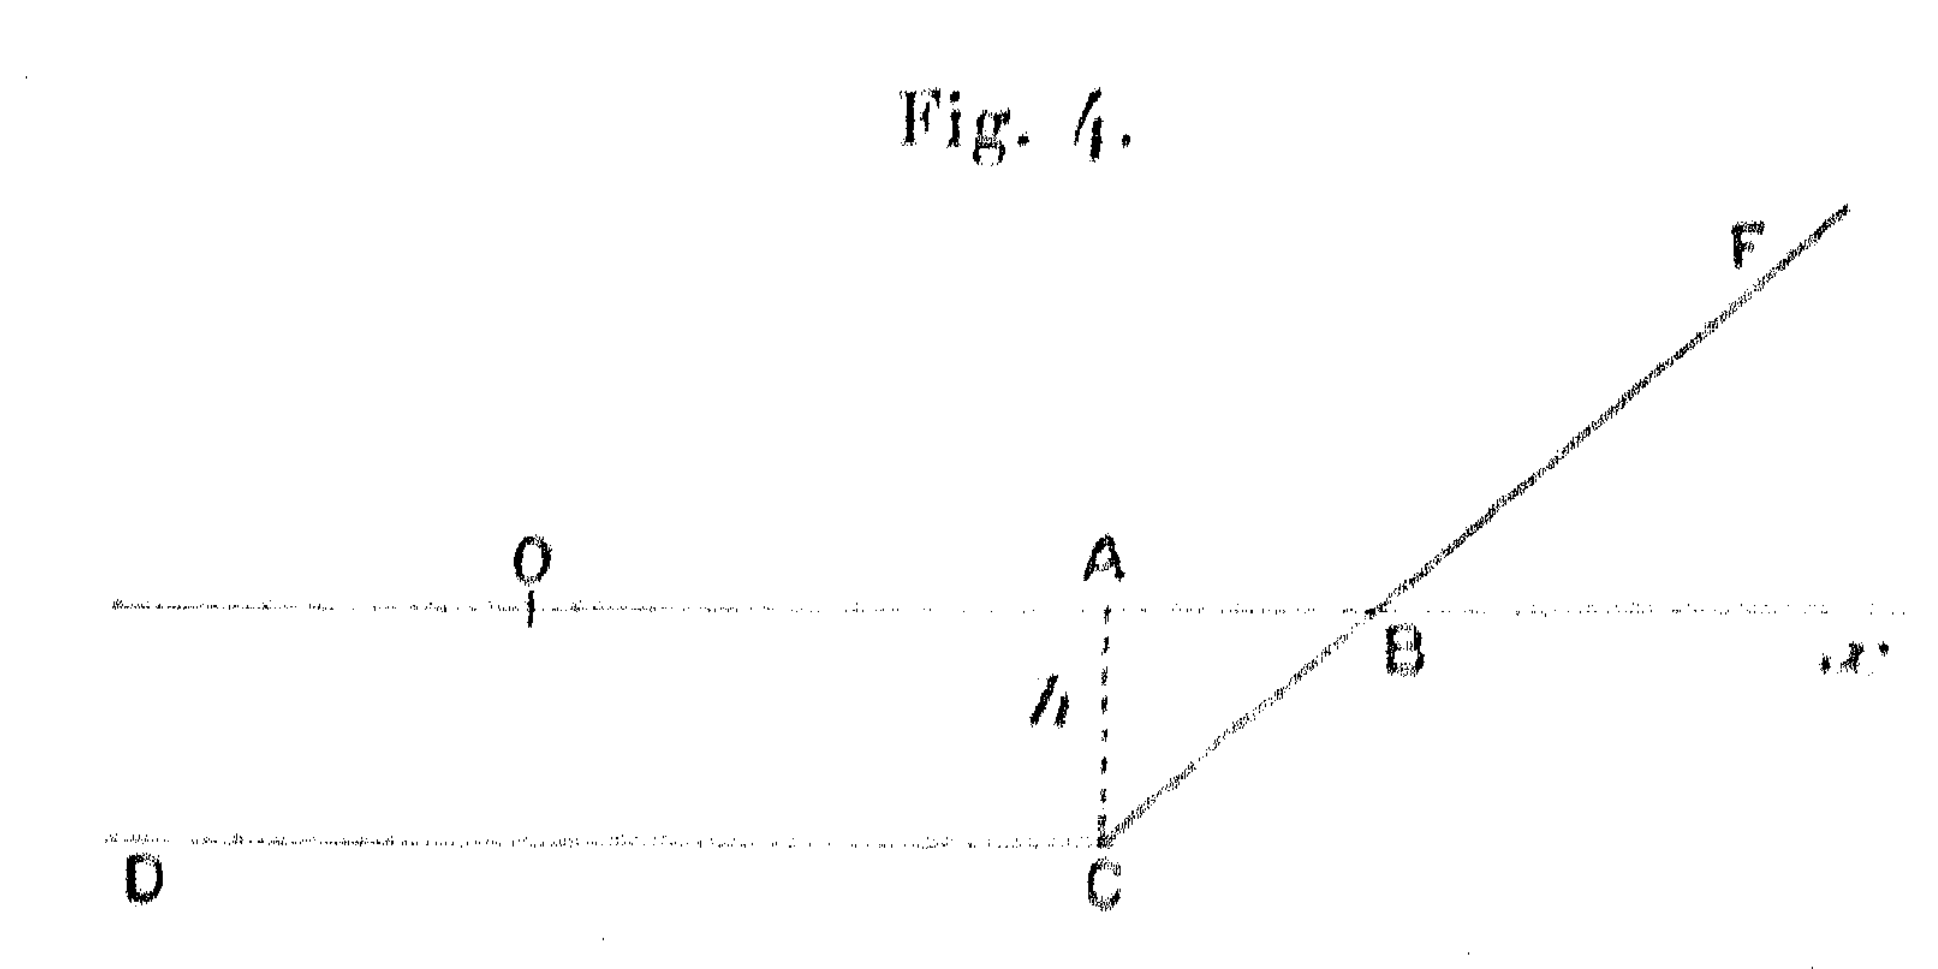
\includegraphics[width=0.5\textwidth]{fig4.png}
\end{center}

Inversement, une \textit{vente à prime} est représentée par une droite brisée en pente négative au-delà du seuil, et plate (gain constant) en dessous. Le vendeur gagne la prime si le marché ne dépasse pas un certain niveau, mais perd au-delà.

Bachelier insiste sur le fait que les marchés à prime permettent de \textit{limiter les pertes}, ce qui les rend attractifs pour certains spéculateurs. Mais cela a un coût ! L'espérance mathématique de la prime est construite de manière à maintenir une neutralité statistique. Il revient sur ce principe plus loin dans sa thèse.

\subsection{Options et stellage}

\begin{quote}
    \emph{« Il est même possible de spéculer uniquement sur la variation absolue du cours, sans égard à la direction dans laquelle elle se produit. »} \\
    — Louis Bachelier, \emph{Théorie de la spéculation}, p. 50
\end{quote}

En complément des opérations simples, le mathématicien introduit (p.~31) ce qu’il appelle des \textit{options} (au sens moderne du terme), c’est-à-dire des instruments hybrides entre le ferme et la prime. En fait, aujourd'hui cela revient à acheter simultanément une option d'achat (call) de prix d'exercice $K$ (le strike), et une option de vente (put) de même strike et même maturity.

Il donne l’exemple d’une \textit{option du double} : une position qui donne droit à deux unités de gain en cas de hausse, mais seulement à une unité de perte en cas de baisse. On parle aujourd’hui d’option asymétrique. De telles structures permettent de moduler le profil de risque selon les anticipations.

De plus, il décrit le \textit{stellage} -- ou \textit{double prime} -- constitué d’une prime à la hausse combinée avec une prime à la baisse. On l’interprète aujourd’hui comme une \textit{stratégie de tunnel, appelée straddle}.

Ce montage donne :
\begin{itemize}
  \item un gain si le cours s’éloigne significativement du cours d’exercice i.e. volatilité grande,
  \item une perte limitée à la somme des deux primes si le cours reste stable.
\end{itemize}

Le stellage est donc une \textit{stratégie directionnellement neutre}, qui mise uniquement sur l’ampleur des variations du cours, et non pas sur la direction du marché.

\begin{center}
    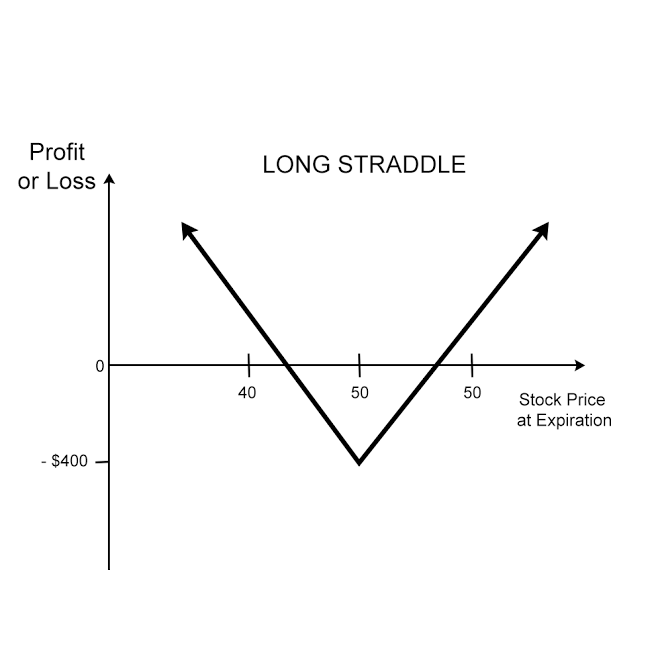
\includegraphics[width=0.4\textwidth]{strad.png}
\end{center}

\medskip

\subsection{Illustrons cela par un exemple}

\begin{itemize}
    \item Prix actuel de l’action : 100~€ ;
    \item Prix d’exercice : $K = 100$~€ ;
    \item Le spéculateur achète :
    \begin{itemize}
        \item un call 100 pour 5~€,
        \item un put 100 pour 5~€.
    \end{itemize}
    \item \textbf{Coût total du straddle} : 10~€.
\end{itemize}

\begin{center}
\begin{tabular}{|c|c|c|c|c|}
\hline
\textbf{Cours à l’échéance} & \textbf{Gain call} & \textbf{Gain put} & \textbf{Gain total} & \textbf{Bénéfice net} \\
\hline
100~€ & 0 & 0 & 0 & \textcolor{red}{--10~€} \\
\hline
110~€ & 10 & 0 & 10 & 0~€ \\
\hline
120~€ & 20 & 0 & 20 & \textcolor{green!60!black}{+10~€} \\
\hline
90~€ & 0 & 10 & 10 & 0~€ \\
\hline
80~€ & 0 & 20 & 20 & \textcolor{green!60!black}{+10~€} \\
\hline
\end{tabular}
\end{center}

Il s’agit d’un pari sur une forte \textit{amplitude des fluctuations} à venir. Dans le modèle de Bachelier, où les variations de prix sont modélisées par un mouvement brownien, le straddle a une valeur croissante avec la \textit{dispersion attendue} des prix, c’est-à-dire leur \textit{variance}. Ce raisonnement annonce les méthodes modernes de valorisation d’options basées sur la \textit{volatilité implicite}.


\bigskip

\noindent
Au terme de cette seconde partie, nous avons compris que cette modélisation des opérations financières est l’un des apports majeurs de Bachelier dans les mathématiques financières que nous connaissons aujourd'hui. Elle permet de visualiser les profils de gains et pertes associés à chaque type d’opération, et prépare le terrain à une analyse probabiliste des stratégies, développée dans les sections suivantes.

\section{Probabilités dans les opérations financières}

\subsection{Probabilités mathématiques et spéculatives}

Le mathématicien précurseur distingue deux types de probabilités dans le contexte des opérations financières :

\begin{itemize}
    \item Les \textit{probabilités mathématiques} sont déterminées \textit{a priori}, sur la base d’hypothèses de symétrie ou de lois connues. Elles sont typiques des jeux de hasard et permettent une modélisation probabiliste rigoureuse.

    \item Les \textit{probabilités spéculatives}, quant à elles, traduisent les anticipations subjectives des agents économiques sur l’évolution future des cours. Ces probabilités sont liées à des jugements personnels basés sur des facteurs économiques, politiques ou psychologiques.
\end{itemize}

Bien que les variations des cours soient imprévisibles, on peut à un instant donné leur associer une \textit{loi de probabilité} décrivant l’état statistique du marché. Dans sa thèse, Bachelier postule que le marché dans son ensemble est \textit{neutre} : il n’anticipe ni la hausse ni la baisse. Cela se traduit mathématiquement par la symétrie de la loi de probabilité autour d’un \textit{cours vrai}.

La fonction de densité de probabilité \( p(x) \) représente la probabilité que le cours relatif, c’est-à-dire l’écart entre le cours effectif et le cours vrai, soit égal à \( x \). Cette densité est symétrique autour de zéro, ce qui s’exprime par :

\[
p(x) = p(-x) \quad \text{pour tout } x \in \mathbb{R}.
\]

Cette propriété, dite de \textit{symétrie ou parité}, traduit l’idée que les fluctuations positives et négatives de même amplitude sont équiprobables, en l’absence de biais directionnel. Elle correspond à un marché \textit{neutre}, où aucune tendance ascendante ou descendante ne domine. On retrouve ici une hypothèse d’\textit{absence d’information privilégiée}, qui anticipe l’idée moderne de \emph{marche aléatoire sans drift}.

On verra dans la section suivante que cette loi est modélisée par une densité normale centrée, solution de l'équation de la chaleur.\\

\subsection{Espérance mathématique et équité du marché}

L’espérance mathématique joue un rôle fondamental dans l’évaluation des jeux de hasard et des opérations financières. Elle est définie comme le produit du gain possible par la probabilité de ce gain. Un jeu est dit \textit{équitable} lorsque son espérance est nulle.

\begin{center}
    \og L’espérance mathématique du spéculateur est nulle. \fg\ p. 34
\end{center}

Ce principe de neutralité permet de garantir que, selon la loi de probabilité admise par le marché à un instant donné, aucune opération n’offre un avantage certain. Ainsi, même une stratégie conditionnelle -- par exemple, vendre dès que le cours dépasse un certain seuil -- a une espérance nulle au regard du marché.

L’hypothèse d’espérance nulle traduit une vision idéale du marché : en l’absence d’information privilégiée, chaque spéculation est un \emph{jeu équitable}, sans avantage structurel. Cette condition se traduit par :

\[
\mathbb{E}[X] = \int_{-\infty}^{+\infty} x \, p(x) \, dx = 0.
\]

Cela signifie que, sur le long terme, le spéculateur ne peut espérer ni gain ni perte en moyenne. Ce principe de neutralité garantit qu’aucune opération, même conditionnelle, ne procure d’avantage certain.

\subsection{Illustrons cela par un exemple}

Considérons un actif valant 100~€ à l’instant initial. Un spéculateur s’attend à ce qu’à l’instant $t = 1$, le cours fluctue autour de cette valeur selon la loi de probabilité simplifiée suivante :

\begin{center}
\begin{tabular}{|c|c|}
\hline
\textbf{Écart $x$ au cours vrai} & \textbf{Probabilité $p(x)$} \\
\hline
$-10$ & $0{,}25$ \\
\hline
$0$   & $0{,}50$ \\
\hline
$+10$ & $0{,}25$ \\
\hline
\end{tabular}
\end{center}

Cette loi est clairement \textit{symétrique} autour de $x=0$ : on a $p(x) = p(-x)$.

Espérance mathématique du gain :
\[
\mathbb{E}[x] = (-10) \cdot 0{,}25 + 0 \cdot 0{,}5 + 10 \cdot 0{,}25 = -2{,}5 + 0 + 2{,}5 = 0
\]

L’espérance est donc nulle : le jeu est \textit{équitable}.

\medskip

Même si le spéculateur élabore une stratégie conditionnelle, par exemple vendre dès que le cours dépasse 110~€, ou acheter en dessous de 90~€, la symétrie des probabilités implique que son \emph{gain espéré reste nul}.
Cela formalise l’idée que \textit{le marché, en l’absence d’information asymétrique}, est un système \textit{neutre et équitable} — tout avantage anticipé est compensé, en moyenne, par un désavantage équivalent.

\medskip

Ce formalisme permet de passer d’un raisonnement spéculatif subjectif à une modélisation mathématique des fluctuations boursières. Même si chaque agent agit sur la base de croyances individuelles, le comportement global du marché peut être décrit par une loi de probabilité objective et continue.

\medskip

\noindent
\textbf{Longue remarque : } il peut sembler paradoxal, voire absurde, de modéliser par des outils mathématiques ce qui relève des croyances subjectives de chaque agent économique. En effet, chaque spéculateur agit en fonction d'informations incomplètes, de jugements personnels et d’intuitions, si bien que prévoir l’avenir des cours semble hors de portée du calcul. C'est aussi une réflexion que je me suis faite. Cependant, la puissance de ces outils mathématiques ne réside pas dans la prédiction d’un cours futur déterminé, mais dans la description statistique du \textit{comportement global} du marché. De la même manière qu'en physique statistique on modélise l’agitation thermique de milliards de particules sans connaître leurs trajectoires individuelles, on peut modéliser l'ensemble des anticipations des agents comme un phénomène aléatoire régulier. On utilise d'ailleurs une équation venant de la physique, celle de la chaleur ! Cette régularité émerge lorsque l’on considère non pas un agent isolé, mais une population d’agents ayant des opinions divergentes qui s’équilibrent en moyenne. C’est ce principe qui justifie l’usage d’une densité de probabilité centrée sur un cours ``neutre'' (le cours vrai), et qui donne sens à une approche probabiliste des marchés.

\subsection{Avantage mathématique}

La situation d’un marché parfaitement équitable, où l’espérance mathématique des spéculateurs est nulle, constitue un cas idéal. Cependant, tous les jeux ou opérations financières ne présentent pas cette symétrie parfaite. En pratique, certaines stratégies offrent une probabilité de gain plus élevée que d’autres, ou bien un gain potentiel supérieur à la perte encourue, sans que l’espérance totale ne soit nécessairement nulle.

\medskip

C’est pourquoi Bachelier introduit une notion complémentaire : celle d’\textit{avantage mathématique}, qui permet de quantifier l'asymétrie d'un jeu (la tendance favorable ou défavorable d’un jeu), même lorsqu’il n’est pas strictement équitable.

\medskip

Le mathématicien définit cet avantage comme le rapport entre l’espérance positive et la somme des espérances positive et négative :
\[
\text{Avantage mathématique} = \frac{\text{espérance positive}}{\text{espérance positive} + \text{espérance négative}}
\]

Cette notion complète celle d’espérance mathématique en évaluant l’asymétrie du jeu : un jeu équitable a un avantage de 1/2, tandis qu’un jeu déséquilibré voit son avantage se rapprocher de 0 ou de 1 selon le sens du déséquilibre.

Enfin, le mathématicien illustre l’égalité des espérances au moyen d’un raisonnement fondé sur les \textit{cours vrais}, qui corrigent les biais liés aux coupons ou aux reports. Par exemple :
\begin{quote}
    \og Les espérances mathématiques de l’acheteur et du vendeur sont nulles quand le report est de 2\% ; [...] si l’on considère ces cours vrais, on peut dire que les espérances mathématiques [...] sont nulles. \fg\ (p. 34)
\end{quote}

Cela justifie, mathématiquement, l’hypothèse de neutralité du marché : même les stratégies fondées sur des options ou des primes sont équitables si on les évalue correctement.

\subsection{Illustrons cela par un exemple}

Considérons un jeu de spéculation dans lequel un spéculateur peut :
\begin{itemize}
    \item gagner 30~€ avec une probabilité de 0{,}3,
    \item perdre 10~€ avec une probabilité de 0{,}7.
\end{itemize}

Ce jeu n’est pas équitable car les probabilités et les montants sont asymétriques.

\medskip

Calcul de l’espérance mathématique :
\[
\mathbb{E}[X] = (30) \cdot 0{,}3 + (-10) \cdot 0{,}7 = 9 - 7 = 2
\]
Le jeu est ici \textit{favorable}, avec une espérance strictement positive.

\medskip

\[
\text{Avantage mathématique} = \frac{\text{espérance positive}}{\text{espérance positive} + \text{espérance négative}}
\]

\medskip

\begin{itemize}
    \item Espérance positive : $30 \cdot 0{,}3 = 9$
    \item Espérance négative : $10 \cdot 0{,}7 = 7$
\end{itemize}

\[
\text{Avantage mathématique} = \frac{9}{9 + 7} = \frac{9}{16} \approx 0{,}5625
\]

\medskip

Ce jeu présente une asymétrie modérée : même si la perte est plus probable, le gain potentiel est plus élevé. L’avantage mathématique est supérieur à 0{,}5, ce qui signifie qu’en moyenne, le jeu est \emph{légèrement favorable} au spéculateur.

Dans un jeu équitable, on aurait un avantage mathématique de $1/2$, tandis qu’un jeu très déséquilibré tendrait vers 0 ou 1 selon qu’il favorise fortement la perte ou le gain.

\bigskip

Au terme de cette troisième partie, nous avons vu comment Bachelier fonde la spéculation sur des principes probabilistes rigoureux, en particulier à travers l’idée que l’espérance mathématique d’un spéculateur est, par défaut, nulle dans un marché équitable. Cette hypothèse de neutralité est ensuite enrichie par la notion d’\emph{avantage mathématique}, qui permet de quantifier les déséquilibres potentiels dans des jeux asymétriques. Ces outils ouvrent la voie à une modélisation fine des opérations financières.

Après avoir posé les fondements probabilistes de la spéculation, Bachelier propose de modéliser \textit{l’évolution temporelle des cours} à l’aide d’une loi de probabilité dépendant du temps. Cette approche marque le passage d’une vision statique des gains attendus à une \textit{description dynamique des fluctuations de marché}.

\section{La dynamique des cours}

\subsection{Loi de probabilité dynamique des cours}

Après avoir étudié la probabilité et l’espérance à un instant donné, Bachelier propose de modéliser l’évolution temporelle des cours par une densité \( p(x,t) \), représentant la probabilité que l’écart du cours effectif au cours vrai soit égal à \( x \) au temps \( t \).

Cette fonction dépend à la fois de la variable \( x \) et du temps \( t \), et doit satisfaire plusieurs propriétés dont la conservation de la masse totale (intégrale égale à 1) et la symétrie :

\[
p(x,t) = p(-x,t).
\]

Le but est alors de déterminer comment cette densité évolue dans le temps, c’est-à-dire comment se comporte $p(x,t)$ lorsque $t$ varie. Pour cela, Bachelier introduit une approche inspirée des méthodes de la physique.

\subsection{Équation de diffusion, de chaleur, de Fourier}

En raisonnant sur la diffusion progressive de la probabilité autour du cours initial, Bachelier établit que la densité $p(x,t)$ doit satisfaire une équation aux dérivées partielles analogue à l’équation de la chaleur :

\[
\frac{\partial p}{\partial t} = \frac{1}{2} \frac{\partial^2 p}{\partial x^2}
\]

\noindent ce qui exprime mathématiquement la manière dont la distribution des cours se diffuse et s’étale dans le temps.

\medskip 

\noindent \textbf{Remarque : } \textit{ cette équation repose sur l’hypothèse que les variations du cours sont le résultat de l’accumulation d’une infinité de petits chocs aléatoires. Le passage à la limite de ce processus conduit à une équation de diffusion, comme dans les mouvements browniens dont voici une illustration :}

\begin{center}
  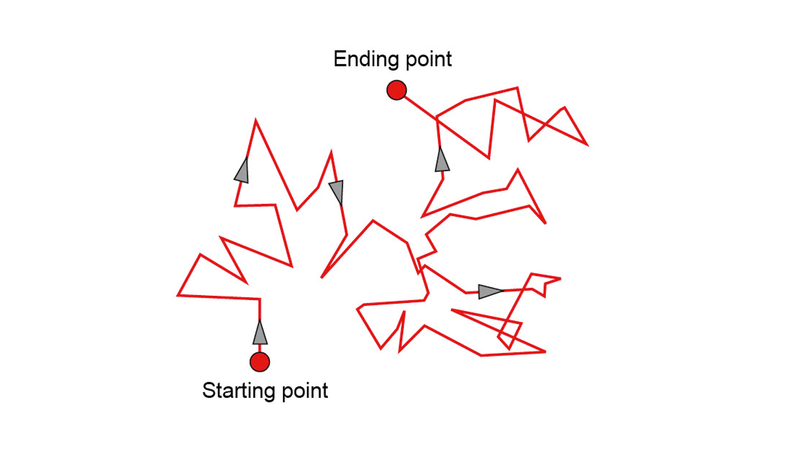
\includegraphics[width=0.6\textwidth]{brownian_motion.png}
\end{center}

\subsection{Solution gaussienne}

La solution fondamentale de cette équation, sous l’hypothèse que le cours est initialement localisé au point $x = 0$, est donnée par la densité normale centrée réduite appelée gaussienne :
\[
p(x,t) = \frac{1}{\sqrt{4\pi t}} \exp\left(-\frac{x^2}{4t}\right)
\]
et dont la très connue représentation graphique est une cloche centrée sur la moyenne :

\begin{center}
  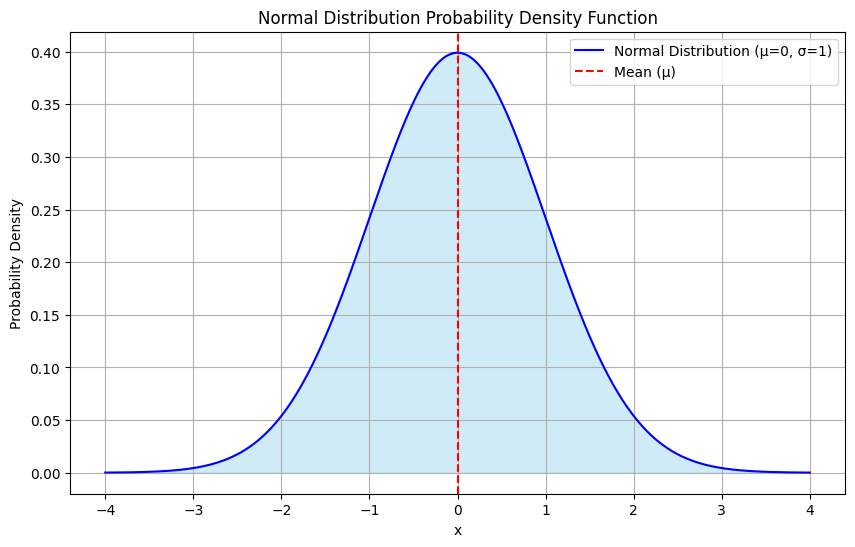
\includegraphics[width=0.6\textwidth]{gaussian_curve.png}
\end{center}

Cette densité garde la propriété de symétrie et montre que l’incertitude sur le cours augmente avec le temps, car l’écart-type est proportionnel à \(\sqrt{t}\).

Cette fonction satisfait les conditions suivantes :
\begin{itemize}
    \item symétrie : $p(x,t) = p(-x,t)$ ;
    \item normalisée : $\int_{-\infty}^{\infty} p(x,t)\, dx = 1$ ;
    \item élargissement avec le temps : la probabilité se diffuse vers les grandes valeurs de $|x|$ ;
    \item tend vers la densité uniforme nulle à l’infini.
\end{itemize}

Cette loi décrit donc la probabilité que le cours ait atteint la valeur $x$ au temps $t$, en supposant qu’il était exactement nul au temps $t = 0$.

\subsection{Illustrons cela par un exemple}

Rappelons que la densité de probabilité \( p(x,t) \) à un instant \( t \) est donnée par :

\[
p(x,t) = \frac{1}{\sqrt{2\pi t}} \exp\left(-\frac{x^2}{2t}\right).
\]

Voici quelques valeurs calculées pour différents \( t \) et \( x \) :

\begin{center}
\begin{tabular}{c|cccc}
\hline
\( t \) & \( p(0,t) \) & \( p(1,t) \) & \( p(2,t) \) & \( p(4,t) \) \\
\hline
1 & 0.399 & 0.242 & 0.054 & 0.0003 \\
4 & 0.199 & 0.176 & 0.121 & 0.021 \\
9 & 0.133 & 0.129 & 0.098 & 0.053 \\
\hline
\end{tabular}
\end{center}

On constate plusieurs points :
\begin{itemize}
  \item À court terme (\( t=1 \)), la densité est très concentrée autour de zéro, ce qui signifie que le cours effectif est très probablement proche du cours vrai — les fluctuations sont faibles.
  \item Avec l’augmentation du temps (\( t=4 ou t=9 \)), la densité s’étale, ce qui traduit une incertitude croissante : il devient plus probable que le cours effectif s’écarte significativement du cours vrai.
  \item Cette diffusion progressive modélise la volatilité naturelle des marchés, où l’écart-type (incertitude) augmente comme \(\sqrt{t}\). Par exemple, la probabilité que l’écart dépasse une valeur élevée (comme 4) est quasi nulle à \( t=1 \), mais devient notable à \( t=4 \) ou \( t=9 \), reflétant le risque croissant sur des horizons plus longs.
\end{itemize}

\subsection{Écart-type et espérance en fonction du temps}

Soit \( X_t \) une variable aléatoire réelle modélisant l’écart entre le cours effectif d’un actif et son cours « vrai » à l’instant \( t \). D’après la modélisation proposée par Bachelier, cette variable suit une loi normale centrée de variance \( 2t \), dont la densité de probabilité est :

\[
p(x,t) = \frac{1}{\sqrt{4\pi t}} \exp\left(-\frac{x^2}{4t}\right)
\]

Cette densité est symétrique par rapport à zéro, ce qui implique que l’espérance mathématique est nulle à tout instant :

\[
\mathbb{E}[X_t] = \int_{-\infty}^{\infty} x\, p(x,t)\, dx = 0
\]

En revanche, la variance de \( X_t \) croît linéairement avec le temps :

\[
\mathbb{V}[X_t] = \int_{-\infty}^{\infty} x^2\, p(x,t)\, dx = 2t
\]

On en déduit que l’écart-type associé à ces fluctuations est :

\[
\sigma(t) = \sqrt{\mathbb{V}[X_t]} = \sqrt{2t}
\]

Cela signifie que les fluctuations typiques du cours croissent comme la racine carrée du temps, ce qui est une caractéristique fondamentale des processus de diffusion. Ainsi, plus on s’éloigne de l’instant initial, plus l’incertitude sur la valeur du cours effectif augmente. On peut donc résumer cette dynamique probabiliste par :

\[
X_t \sim \mathcal{N}(0,\, 2t)
\]

où \( \mathcal{N}(0, 2t) \) désigne la loi normale de moyenne nulle et de variance \( 2t \). Cette modélisation rend compte de l’aléa inhérent aux marchés, tout en permettant une description quantitative précise de l’évolution des cours.

Cette approximation par la loi normale est issue du \textit{théorème central limite} que nous ne détaillerons pas ici (il a été détaillé dans un autre papier). Si l’on suppose que les variations infinitésimales du cours à chaque instant sont indépendantes, de faible amplitude, et symétriques, alors la somme de ces petites variations sur un intervalle de temps \( t \) tend vers une loi normale lorsque le nombre de pas devient très grand. Ce raisonnement est une approximation naturelle de nombreux phénomènes aléatoires dans lesquels aucune direction n’est privilégiée.

En d’autres termes, si l’on modélise l’évolution du cours par un processus aléatoire à pas discrets, la variable aléatoire \( X_t \), représentant l’écart cumulé au cours vrai après un grand nombre d’interactions de marché, suit approximativement une loi gaussienne. C’est cette limite continue que Bachelier formalise dans sa thèse, en posant directement que \( X_t \sim \mathcal{N}(0, 2t) \), dont la densité satisfait l’équation de diffusion.

\bigskip

C’est dans ce cadre qu’intervient l’analogie avec la \textit{diffusion thermique}, et que se précise l’idée d’un mouvement aléatoire continu du cours, que Bachelier anticipe sous la forme d’un processus que l’on nommera plus tard \textit{mouvement brownien}.


\section{Applications aux options et primes} % TODO Finir ce papier + faire un papier sur le théorème central limite, la loi gausienne et loi normale (approximation etc) + entourer les grosses formules par \boxed{}

\subsection{Prime simple : calcul et probabilité de réussite}

Une \textit{prime simple} -- ou bien une option européenne d'achat ou de vente -- permet à son détenteur de profiter d’un gain conditionnel à la réalisation d’un scénario favorable, tout en limitant ses pertes au montant initialement payé, appelé la \textit{prime}. 

Bachelier modélise l'achat d'une prime à la hausse, de seuil \( a > 0 \), qui donne un gain égal à \( x - a \) lorsque le cours effectif \( x \) dépasse ce seuil, et nul sinon. Le cours est ici centré autour du \textit{cours vrai}, de sorte que la densité \( p(x,t) \) est symétrique et centrée sur zéro.

\paragraph{Espérance mathématique du gain.}

La valeur attendue du gain pour l’acheteur de la prime est donnée par l'intégrale :

\[
\mathbb{E}[\text{gain}] = \int_a^{\infty} (x - a)\, p(x,t)\, dx
\]

Mais selon le \textit{principe d’équité du marché}, cette espérance doit être nulle si la prime est justement valorisée. En effet, si le détenteur de la prime a une espérance de gain non nulle, cela signifie qu’un arbitrage est possible, ce qui contredit l'hypothèse de neutralité du marché. Cela revient à imposer :

\[
\mathbb{E}[\text{gain}] - a = 0 \quad \Rightarrow \quad a = \int_0^{\infty} x\, p(x,t)\, dx
\]

Autrement dit, le montant de la prime est exactement égal à l’espérance positive d’un achat ferme : c’est la moyenne des gains potentiels, pondérés par la probabilité qu’ils se réalisent. Cela établit un lien direct entre le prix de l’option et l’intégrale de la partie positive de la densité.

\paragraph{Probabilité de succès.}

Bachelier calcule également la \textit{probabilité de succès} d’une prime simple, c’est-à-dire la probabilité que le cours effectif dépasse le seuil \( a \), ce qui permet à l’option de s’exercer. Il montre que cette probabilité est constante et indépendante du temps :

\[
\mathbb{P}(X_t > a) = \int_a^{\infty} p(x,t)\, dx = 0{,}345
\]

Ce résultat découle du fait que la densité \( p(x,t) \) est une gaussienne \( \mathcal{N}(0, 2t) \), et que \( a \) est fixé de sorte que :

\[
\int_0^{\infty} x\, p(x,t)\, dx = a
\]

Le seuil \( a \) correspond à une fraction fixe de l'écart-type \( \sqrt{2t} \), ce qui implique que la probabilité d’atteinte du seuil reste constante quelle que soit l’échelle de temps. Cela reflète l’idée fondamentale que le marché « ajuste » la prime en fonction de l’horizon temporel, de sorte que l’équité soit préservée.

\paragraph{Interprétation.}

Ce modèle permet de fixer un prix juste à une option dans un marché symétrique, sans biais directionnel. Même si la probabilité de gain est inférieure à 50\% (ici 34,5\%), le montant du gain potentiel compense cette asymétrie, rendant le jeu équitable.

\subsection{Écart probable et valeur attendue}

L’\textit{écart probable} est défini comme la valeur seuil \( a \) telle que le cours ait une chance sur deux de s’en écarter en valeur absolue à l’échéance. Autrement dit, il s’agit de la borne symétrique autour du cours moyen (ici centré en 0) qui capture 50\,\% de la probabilité :

\[
\mathbb{P}(|X_t| < a) = 0{,}5
\]

Puisque \( X_t \sim \mathcal{N}(0, 2t) \), la densité est symétrique et la distribution des écarts suit une gaussienne centrée. On peut donc exprimer \( a \) sous la forme :

\[
a = \lambda \sqrt{2t}, \quad \text{où } \lambda \approx 0{,}674
\]

Cette constante \( \lambda \) correspond à la médiane de la loi normale centrée réduite en valeur absolue : 50\,\% des réalisations sont alors comprises entre \( -a \) et \( +a \). L’écart probable est ainsi un indicateur de dispersion plus robuste que l’écart-type, car il se fonde sur la médiane et non sur la moyenne quadratique.

Dans le cas d’une prime simple de valeur \( a \), Bachelier calcule que la \textit{valeur moyenne des gains} lorsque le seuil est franchi (c’est-à-dire l’espérance conditionnelle positive) vaut :

\[
\mathbb{E}_+(X_t > a)[X_t - a] = 0{,}58 \cdot a
\]

Ainsi, le prix de la prime peut être vu comme le résultat d’un calcul d’espérance, pondéré uniquement sur les scénarios favorables, ce qui reflète à nouveau le principe d’équité du marché : le coût d’une stratégie risquée est exactement égal à la valeur attendue de ses gains.

\subsection{Double prime et loi des écarts}

Détaillons ce que nous avions énoncé dans la partie \textbf{3.2 Options et stellage}... Nous avions vu que la \textit{double prime} (ou \textit{stellage}) combine une prime à la hausse et une prime à la baisse. Le preneur paie deux primes de valeur $a$ et ne gagne que si le cours final s’écarte significativement (vers le haut ou vers le bas). Cette stratégie est neutre vis-à-vis de la direction du marché mais sensible à la \textit{volatilité}.

Sa valeur correspond à la somme des deux espérances positives de chaque prime :
\[
\text{Valeur du stellage} = 2a = \int_{-\infty}^{-a} (-x - a)\, p(x)\, dx + \int_a^{\infty} (x - a)\, p(x)\, dx
\]

Bachelier montre que si le marché sous-évalue l’écart entre les primes et le cours ferme, il est possible de combiner plusieurs options de manière à construire une stratégie \textit{arithmétiquement gagnante} (p. 30). Il donne ainsi l’exemple d’un arbitrage entre différentes primes si la loi des écarts n’est pas respectée.

\subsection{Comprendre cette stratégie de \textit{straddle} par un exemple...}

Supposons que :
\begin{itemize}
    \item le cours vrai est de \( 100\,euros \),
    \item les primes à la hausse et à la baisse ont un seuil de \( 5\,euros \) autour du cours vrai : seuils \( 95\,euros \) et \( 105\,euros \),
    \item chaque prime coûte \( 2\,euros \),
    \item le coût total du straddle est donc \( 4\,euros \).
\end{itemize}

À l’échéance, les gains dépendent du cours effectif :

\begin{center}
\begin{tabular}{c|c|c|c|c}
\hline
Cours final & Gain call & Gain put & Gain total & Gain net \\
\hline
100\,€ & 0 & 0 & 0 & -4\,€ \\
106\,€ & 1 & 0 & 1 & -3\,€ \\
120\,€ & 15 & 0 & 15 & \textbf{+11\,€} \\
94\,€ & 0 & 1 & 1 & -3\,€ \\
80\,€ & 0 & 15 & 15 & \textbf{+11\,€} \\
\hline
\end{tabular}
\end{center}

\paragraph{Interprétation.}

Lorsque le marché reste stable autour du cours vrai, les deux primes expirent sans valeur, et l’acheteur du straddle perd l’intégralité de la prime payée. En revanche, si le cours fluctue fortement dans un sens ou dans l’autre, l’une des deux options devient rentable et permet de compenser (et même dépasser) le coût initial. Le straddle est donc une stratégie \textit{neutre directionnellement}, mais \textit{sensible à la volatilité}.

\subsection{Formule intégrale et interprétations}

L’évaluation des \textit{primes} repose sur des intégrales qui expriment des quantités économiques de manière mathématique. Deux intégrales fondamentales apparaissent dans la thèse de Bachelier :

\[
\int_a^{\infty} (x - a)\, p(x,t)\, dx
\quad \text{et} \quad
\int_a^{\infty} p(x,t)\, dx
\]

Elles représentent respectivement :
\begin{itemize}
    \item la \textbf{valeur attendue} du gain pour un acheteur de prime, c’est-à-dire le gain moyen lorsqu’il y a exercice de l’option (lorsque le cours dépasse le seuil \( a \)) ;
    \item la \textbf{probabilité de succès}, c’est-à-dire la probabilité que le cours effectif dépasse le seuil d’exercice \( a \).
\end{itemize}

Ces intégrales reposent sur la densité de probabilité \( p(x,t) \), qui, dans le modèle de Bachelier, est une loi normale centrée de variance \( 2t \). Autrement dit, \( p(x,t) \) décrit la manière dont les cours peuvent s’écarter du cours « vrai » au temps \( t \), avec une probabilité plus forte autour de zéro, et plus faible aux extrémités.

\paragraph{Croissance dans le temps.}

Bachelier démontre que le montant d’une prime simple équitable, que l’on note \( a(t) \), dépend du temps de manière proportionnelle à la racine carrée du temps :

\[
a(t) \propto \sqrt{t}
\]

Le symbole \( \propto \) signifie \og est proportionnel à \fg, c’est-à-dire qu’il existe une constante \( k \) telle que :

\[
a(t) = k \cdot \sqrt{t}
\]

Cela reflète le fait que plus le temps passe, plus l’incertitude sur l’évolution du cours augmente, ce qui accroît la valeur des options. En effet, dans le cadre d’un mouvement brownien, l’écart-type croît comme \( \sqrt{t} \), ce qui élargit la zone dans laquelle le cours peut s’écarter, augmentant la valeur potentielle d’une option.

\bigskip

Ces formules constituent les premières tentatives rigoureuses de valorisation d'options, bien avant le célèbre modèle de Black-Scholes (1973). Dans le modèle de Bachelier, les cours suivent un processus gaussien \textit{additif} : les variations s'ajoutent au cours de façon aléatoire avec une variance croissante. Cela conduit à une distribution normale des variations de prix.
Le modèle moderne de Black-Scholes lui suppose un mouvement brownien \textit{géométrique} où les rendements sont aléatoires, pas les prix eux-mêmes, mais repose sur une intuition similaire : le \textit{prix d'une option équitable} est donné par la \textit{valeur espérée de ses gains}, en tenant compte de la probabilité de succès.


\section{Vision moderne du modèle de Bachelier}
%TODO
\end{document}